\documentclass[a4paper]{article}
\usepackage{titling}
\usepackage{amsmath}
\usepackage{mathtools}
\pagenumbering{gobble}
\usepackage{graphicx}
\usepackage{hyperref}
\usepackage[bottom]{footmisc}
\usepackage{booktabs}
\usepackage{sectsty}
\usepackage{wrapfig}
\sectionfont{\centering}
\usepackage{array}
\usepackage{subfig}
\usepackage{paralist}
\usepackage{verbatim}
\usepackage{subfig}
\usepackage{algorithm}
\usepackage{algpseudocode}
\usepackage{fancyvrb}
\usepackage{multirow}
\usepackage{rotating}
\usepackage{pgfplots}
\usepackage{wrapfig}
\pgfplotsset{width=4cm,compat=1.9}
\usepackage{fancyhdr}
\usepackage{float}
\usepackage{hyperref}
\usepackage{amsfonts}
\usepackage[utf8]{inputenc}
\usepackage[scaled]{helvet}
\usepackage{titlesec}
\usepackage{lipsum}
\usepackage[margin=0.5in]{geometry}
\renewcommand\familydefault{\sfdefault} 
\usepackage[T1]{fontenc}

\usepackage{biblatex} %Imports biblatex package
\addbibresource{references.bib} %Import the bibliography file

\setlength{\droptitle}{-6em}

\author{}
\date{}
\title{Monthly Summary Report: January 2023\vspace{-3.5em}}

\begin{document}
\maketitle

\noindent This monthly summary report provides an overview of the earthquake activity for the North-East of the Netherlands, using data gathered from an \href{https://cdn.knmi.nl/knmi/map/page/seismologie/all_induced.json}{API} provided by the Royal Dutch Meteorological Society, which contains earthquake recordings in the region. These recordings comprise the earthquake types, places, locations, coordinates, dates \& times and magnitudes (assessed using the unit of local magnitude $Ml$). This report analyses data from 2022-02-01 to 2023-01-31 and has two distinct objectives; to select a value for the magnitude of completion based on the data, and to draw a comparison between the earthquake activity in the last month and the average seismic behaviour in the 11 months preceding that.

\section*{\centering\textnormal{Data-Driven Selection of the Magnitude of Completion}}
\begin{wrapfigure}{l}{0.6\textwidth}
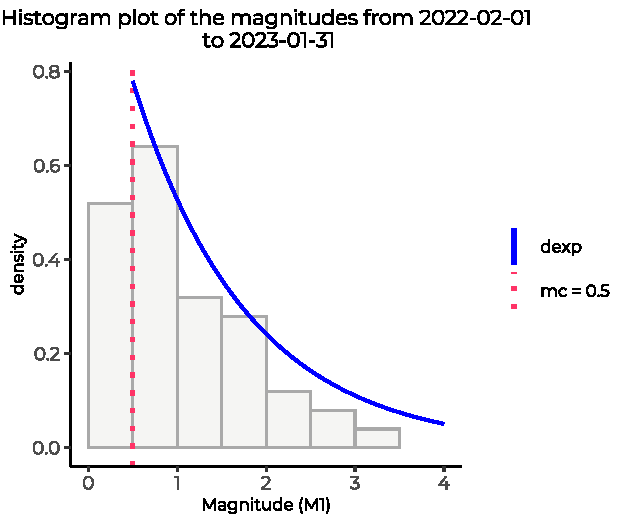
\includegraphics[width=0.9\linewidth]{01-01-hist-mc.pdf} 
\caption{}
\label{fig:wrapfig}
\end{wrapfigure}
Some earthquakes with magnitudes below a certain level $m_c$ (the magnitude of completion) might not be recorded - the further they fall below $m_c$, the more likely they are to be missed. Assuming an Exponential($\beta$) distribution for earthquake magnitudes, any deviations from this model are attributed to incomplete observation. For the entire time period, a conservative estimate of $m_c$ is 1.5$Ml$, though it decreases over time. To find an estimate of $m_c$, namely $\hat m_c$, a histogram of all the magnitude values is plotted, with number of bins k according to Scott's rule \cite{hist}, i.e. k = $3.5sd(x)n^{-\frac{1}{3}}$, where sd(x) the standard deviation of the data x and n the sample size. The estimate $\hat m_c$ adopted is the left border of the bin with the highest number of counts; this approach is justified by the decreasing property of the Exponential density function. Thus, we keep only the magnitudes bigger than $\hat m_c$. The histogram can be seen in Figure \ref{fig:wrapfig}, with the estimated value of $m_c$ and the fitted density curve of the Exponential, computed using the MLE of $\beta$, $\hat \beta = \frac{1}{\bar x}$ (where $\bar x$ the sample mean of the completed magnitudes). Indeed, the data that are deemed complete by the proposed estimate seem to closely follow the Exponential($\hat \beta$) density curve. However, this approach needs to be validated further; to this end, two Q-Q plots are used (Figures \ref{fig2} \& \ref{fig3}). The left one presents the sample quantiles of our magnitude data against the theoretical quantiles of the exponential distribution the data would follow if it were exponential, i.e. exp($\tilde \beta$), with $\tilde \beta = \frac{1}{\bar y}$ and y all the magnitudes. The right presents the sample \& theoretical quantiles of the completed magnitudes, meaning we only use magnitudes bigger than $m_c$ for the data and the MLE. Because of this, the value of $\hat m_c$ was subtracted from all observations, so the line begins at the origin; this is why the new blue dotted line is also 1.5 - $\hat m_c$. The closer the scatterplot follows the plotted qqline, the better the fit for the distribution. We observe that, while in Figure \ref{fig2}, the points underneath the $m_c$ line seem to deviate from the line y = x, after only keeping magnitudes bigger than $\hat m_c$, the points follow the straight line closely; the only discrepancy visible is that after the blue dotted line, which corresponds to the conservative estimate of $m_c$ equal to 1.5$Ml$, above which observations are certain to be complete.\\

\begin{figure}[H]
  \centering
  \begin{minipage}[b]{0.45\textwidth}
    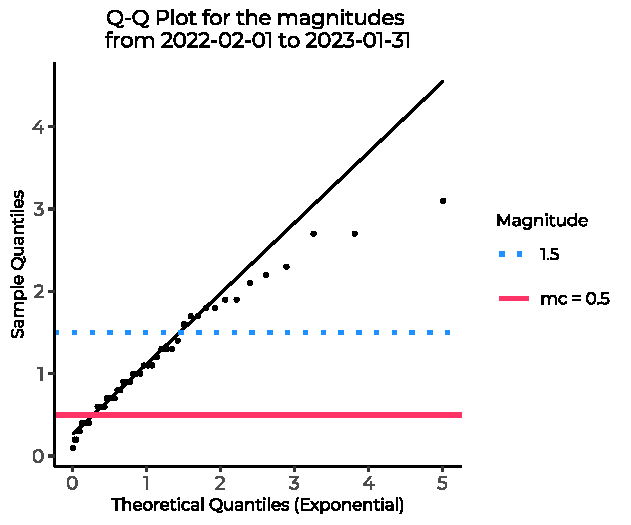
\includegraphics[width=\textwidth]{01-02-qqplot-1.pdf}
    \caption{}
    \label{fig2}
  \end{minipage}
  \hfill
  \begin{minipage}[b]{0.45\textwidth}
    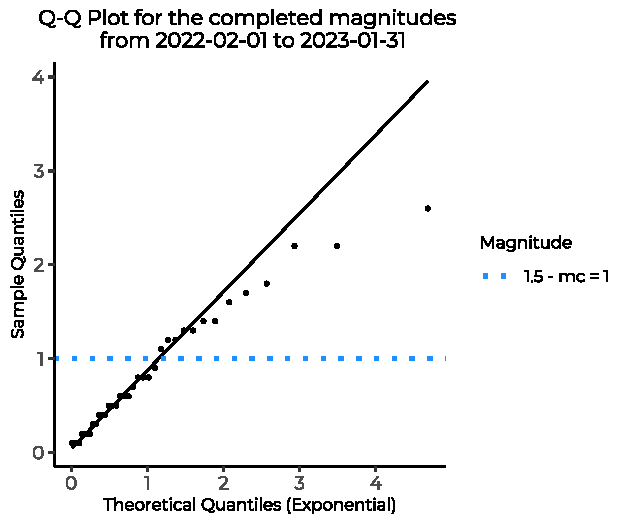
\includegraphics[width=\textwidth]{01-03-qqplot-2.pdf}
    \caption{}
    \label{fig3}
  \end{minipage}
\end{figure}
\clearpage
\section*{\centering\textnormal{Comparative Analysis of Earthquake Activity: Last Month \& Previous 11 Months}}
This report will now focus on investigating the last month's earthquake activity for the North-East of the Netherlands, compared to the average activity in the 11 months preceding that. The API data are now cleaned to contain only completed observations of the last 12 months, using the previously estimated value for the magnitude of completion $m_c$. The aim is to gain a comprehensive overview of the seismic landscape in the past year, as well as how it changes over time \& location. \\

\noindent The analysis begins by presenting two bubble plots corresponding to the last month (Figure \ref{fig4}) and the prior 11 months (Figure \ref{fig5}). These encompass the longitude, latitude and location names, as well as the earthquake magnitudes and counts. However, for the right bubble plot, the \textit{average} of longitude, latitude \& magnitudes where used. In the last month (January 2023), there's a record of 2 earthquakes, both of which took place in \textbf{Garsthuizen} with magnitudes 1.3$Ml$ \& 1.8$Ml$ respectively. This is surprising, as in the 11 months prior to that, Garsthuizen was the epicenter of only one earthquake with a relatively low magnitude (below 1$Ml$). Similarly, \textbf{Froombosch} and \textbf{Lageland} were also struck by 1 earthquake, however their respective \textbf{magnitudes were the highest} overall (over 1.5$Ml$). On the contrary, \textbf{Wirdum} and \textbf{Uithuizen} seem to suffer from the  \textbf{most earthquakes} out of all locations, the magnitudes of which are moderately high (close to 1.5$Ml$). The rest of the locations have varying earthquake counts, however their mean magnitudes all remain below 1.5$Ml$. \\


\begin{figure}[H]
  \centering
  \begin{minipage}[b]{0.49\textwidth}
    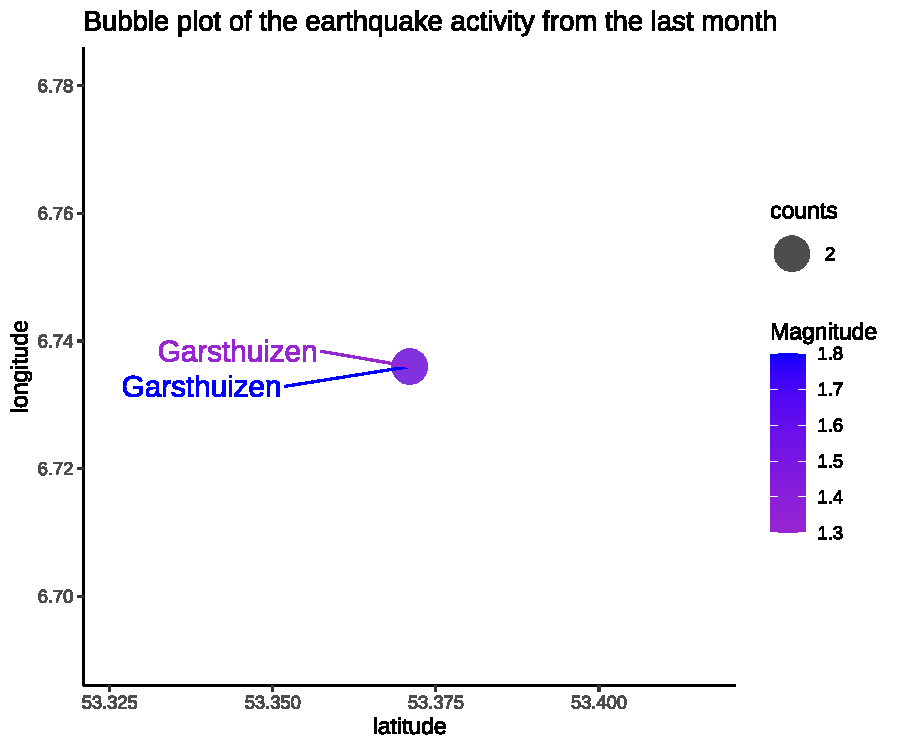
\includegraphics[width=\textwidth]{02-01-bubble-plot-1.pdf}
    \caption{}
    \label{fig4}
  \end{minipage}
  \hspace{0.1em}
  \begin{minipage}[b]{0.49\textwidth}
    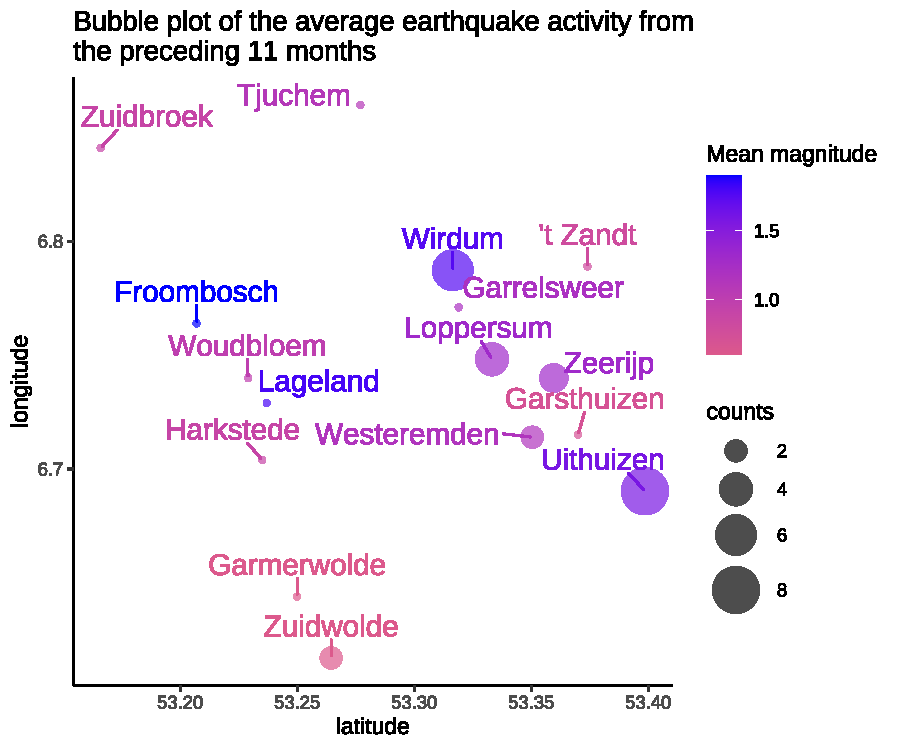
\includegraphics[width=\textwidth]{02-02-bubble-plot-2.pdf}
    \caption{}
    \label{fig5}
  \end{minipage}
\end{figure}

\noindent The subsequent analysis delves into the monthly seismic activity over the entire region of interest, which is summarised in Table \ref{tab1}. The average counts per month before January 2023 is 3, while the average overall magnitude is 1.11$Ml$. Consequently, the month of January 2023 had less earthquakes than average (2), but they were more intense than usual (with magnitudes 1.3$Ml$ \& 1.8$Ml$). The highest earthquake counts were recorded in the months of September (7), October (7) and December (6), with the \textbf{biggest overall magnitude of 3.1$Ml$} also taking place in October. Following in highest magnitudes (2.7$Ml$) are the months of April and September. On the contrary, in February no earthquakes were recorded at all.\\

%%%%%%%%%%%%%%%%%%%% PLEASE REPLACE WITH NEW TABLE HERE %%%%%%%%%%%%%%%%%%%%%%%%%%%%%%%%%%%
% latex table generated in R 4.0.3 by xtable 1.8-4 package
% Mon May 15 17:13:54 2023
\begin{table}[ht]
\centering
\begin{tabular}{rrrrrrrrrrrrr}
  \hline
 & Jan & Feb & Mar & Apr & May & Jun & Jul & Aug & Sep & Oct & Nov & Dec \\ 
  \hline
counts & 2.00 & 0.00 & 2.00 & 4.00 & 2.00 & 2.00 & 2.00 & 2.00 & 7.00 & 7.00 & 1.00 & 6.00 \\ 
  min mag & 1.30 & 0.00 & 0.70 & 0.60 & 0.60 & 0.70 & 0.90 & 1.30 & 0.70 & 1.00 & 0.60 & 0.60 \\ 
  mean mag & 1.55 & 0.00 & 1.40 & 1.40 & 1.20 & 0.80 & 1.00 & 1.60 & 1.44 & 1.61 & 0.60 & 1.18 \\ 
  max mag & 1.80 & 0.00 & 2.10 & 2.70 & 1.80 & 0.90 & 1.10 & 1.90 & 2.70 & 3.10 & 0.60 & 1.90 \\ 
   \hline
\end{tabular}
\caption{Table showing the monthly earthquake activity for the past
                       12 months.} 
\label{tab1}
\end{table}
%%%%%%%%%%%%%%%%%%% END OF TABLE %%%%%%%%%%%%%%%%%%%%%%%%%%%%%%%%%%%%%%%%%%%%%%%%%%%%%%%%%%


\noindent It is worth reiterating that magnitudes are measured in units of local magnitude $Ml$; as such, values less than 1$Ml$ to 2.9$Ml$ (microearthquakes) are imperceptible to humans and exhibit minimal potential for causing significant damage, though they are detectable by seismometers \cite{britannica}. On the other hand, earthquakes with magnitudes between 3$Ml$ and 3.9$Ml$ (minor earthquakes) may be felt by individuals in close proximity to the epicenter, but they also don't cause substantial infrastructure damage or pose significant risks \cite{britannica}. Throughout the last 12 months (February 2022 - January 2023), there were no recorded instances of earthquakes exceeding a magnitude of 4$Ml$. In the month of January 2023, only microearthquakes were recorded. During the preceding 11 months, \textbf{a single earthquake} out of a total of 35 recorded seismic events was classified as \textbf{minor}, while the remaining were categorised as \textbf{microearthquakes}. Consequently, the North-East region of the Netherlands remained unaffected by any high-risk earthquakes throughout the past 12 months. The ubiquity of microearthquakes suggests that the overall seismic activity does not raise significant concerns.

\printbibliography
\end{document}

